% Task 6: a piece of a CT log and Bob's records. Values from Task6/ (python3, Task6/ctlog.py, 2026-11-26).
% CHECKED: the nine entries (issued, CA, names) and the SHA-256 fingerprints 5f1d8b540c1665af... and b2acc6775a289bc0...
%   of the two certificates in my_orders.txt; caa.txt: bob.example. CAA 0 issue "trusty-ca.example"
\documentclass[12pt,tikz,border=6pt]{standalone}
% Shared preamble of the task figures of Lecture 12.
% The colours and styles are copied from the preamble of ../main.tex (keep them in sync).
% Colour mapping of Lecture 12:
%   S1 indigo: Alice (signs code and mail; in HTTPS the client)   S2 pink: Mallory, a fake certificate
%   S3 violet: a certificate                  S4 amber: a private key (black text)
%   S5 teal: Bob (checks code and mail; in HTTPS owns the website)   S6 brown: a CA or a TSA
\usepackage{lmodern}
\usepackage[T1]{fontenc}
\renewcommand{\familydefault}{\sfdefault}
\usepackage{amsmath,amssymb}
\usepackage{xcolor}
\usepackage{fontawesome5}
\usetikzlibrary{arrows.meta, calc, positioning, fit, decorations.pathreplacing, backgrounds, shadows}

\definecolor{DeepBlue}{HTML}{283593}
\definecolor{AccentOrange}{HTML}{EB5A14}
\definecolor{LightGray}{HTML}{F5F6FA}
\definecolor{sIndigo}{HTML}{5C6BC0}
\definecolor{sPink}{HTML}{EC407A}
\definecolor{sViolet}{HTML}{7E57C2}
\definecolor{sAmber}{HTML}{FFB300}
\definecolor{sTeal}{HTML}{26A69A}
\definecolor{sBrown}{HTML}{8D6E63}
\definecolor{sPinkText}{HTML}{C2185B}
\definecolor{sAmberText}{HTML}{A06A00}
\definecolor{sTealText}{HTML}{00796B}
\definecolor{aExec}{HTML}{43A047}
\definecolor{aRead}{HTML}{1E88E5}
\definecolor{aWrite}{HTML}{E53935}
\definecolor{nInk}{HTML}{37474F}
\definecolor{nLine}{HTML}{90A4AE}
\definecolor{nLight}{HTML}{CFD8DC}
\definecolor{nFill}{HTML}{ECEFF1}
\definecolor{nIdle}{HTML}{E0E0E0}

\tikzset{
  hw/.style={draw=nLine, thick, fill=nFill, text=nInk, rounded corners=3pt, align=center, inner sep=4pt},
  hwmain/.style={draw=nInk, thick, fill=nInk, text=white, rounded corners=3pt, align=center, inner sep=4pt},
  container/.style={draw=nLine, thick, dashed, rounded corners=5pt},
  actor/.style={fill=#1, draw=#1, text=white, rounded corners=3pt, align=center, font=\small\bfseries, inner sep=5pt},
  actorlight/.style={fill=#1!15, draw=#1, thick, text=nInk, rounded corners=3pt, align=center, inner sep=5pt},
  person/.style={circle, fill=#1, draw=#1, text=white, minimum size=1.1cm, font=\Large, inner sep=0pt},
  data/.style={-{Stealth}, very thick, nInk},
  flow/.style={-{Stealth}, very thick, DeepBlue},
  annot/.style={draw=AccentOrange, line width=1.6pt, rounded corners=3pt},
  note/.style={font=\small, text=nInk},
  % a certificate card: violet frame, light violet fill
  cert/.style={draw=sViolet, thick, fill=sViolet!10, text=nInk, rounded corners=3pt, align=left, inner sep=5pt,
    font=\small},
  fakecert/.style={draw=sPink, thick, fill=sPink!10, text=nInk, rounded corners=3pt, align=left, inner sep=5pt,
    font=\small},
  keybox/.style={draw=sAmber, thick, fill=sAmber!25, text=black, rounded corners=3pt, align=center, inner sep=4pt},
  cabox/.style={fill=sBrown, draw=sBrown, text=white, rounded corners=3pt, align=center, font=\small\bfseries, inner sep=5pt},
  byte/.style={draw=nLine, thick, fill=white, text=nInk, font=\ttfamily\small,
    minimum width=0.72cm, minimum height=0.58cm, inner sep=1pt, rounded corners=1.5pt},
  chg/.style={byte, fill=AccentOrange!18, draw=AccentOrange, line width=1.4pt, font=\ttfamily\small\bfseries},
  rowlabel/.style={font=\small\bfseries, text=nInk, anchor=east},
}
\newcommand{\ok}{\textcolor{aExec}{\faCheck}}
\newcommand{\nok}{\textcolor{aWrite}{\faTimes}}
\newcommand{\qm}{\textcolor{AccentOrange}{\textbf{?}}}
% a file icon with a name under it: \fileicon{node name}{position}{label}
\newcommand{\fileicon}[3]{%
  \node[text=nInk, font=\fontsize{26}{28}\selectfont] (#1) at (#2) {\faFile*[regular]};
  \node[font=\scriptsize\ttfamily, text=nInk, below=0.02cm of #1] {#3};}

\begin{document}
\pagecolor{white}
\begin{tikzpicture}[>=Stealth]
  \node[font=\small\bfseries, text=nInk, anchor=west] at (-0.2,0.75) {\faScroll\ ct\_log.pem: a piece of a public CT log, oldest first};
  \foreach \k/\dt/\ca/\nm in {
      0/2026-10-02/Green CA/{bakery.example, www.bakery.example},
      1/2026-10-05/Trusty CA/{bob.example, www.bob.example},
      2/2026-10-09/Green CA/{carol.example},
      3/2026-10-14/Trusty CA/{api.bob.example},
      4/2026-10-21/Green CA/{bob.example.mallory.example},
      5/2026-10-25/Trusty CA/{dave.example, mail.dave.example},
      6/2026-11-02/Shady CA/{bob.example, www.bob.example},
      7/2026-11-06/Trusty CA/{login.bob.example},
      8/2026-11-09/Shady CA/{mallory.example}} {
    \pgfmathsetmacro{\y}{-0.62*\k}
    \node[cert, minimum width=10.4cm, minimum height=0.52cm, inner sep=2pt, anchor=west] at (0,\y) {};
    \node[font=\scriptsize\ttfamily, text=nInk, anchor=west] at (0.1,\y) {\dt};
    \node[font=\scriptsize, text=nInk, anchor=west] at (2.0,\y) {\ca};
    \node[font=\scriptsize\ttfamily, text=nInk, anchor=west] at (3.8,\y) {\nm};
    \node[circle, draw=AccentOrange, thick, fill=white, minimum size=0.42cm, inner sep=0pt, font=\bfseries\scriptsize,
      text=AccentOrange] at (10.75,\y) {?};
  }
  % ---------- Bob, the domain owner ----------
  \node[person=sTeal] (a) at (14.4,0.2) {\faUser};
  \node[font=\small\bfseries, text=sTeal, below=0.05cm of a] {Bob};
  \node[font=\scriptsize, text=nInk, anchor=north] at (14.4,-0.95) {owns \texttt{bob.example}};
  \node[hw, anchor=north, text width=5.0cm, align=left, font=\scriptsize] (o) at (14.4,-1.45)
    {\textbf{my\_orders.txt}: SHA-256 fingerprints\\ \texttt{5f1d8b540c1665af\ldots}\\ \texttt{b2acc6775a289bc0\ldots}};
  \node[hw, anchor=north, text width=5.0cm, align=left, font=\scriptsize] (c) at (14.4,-3.0)
    {\textbf{caa.txt}: his DNS record\\ \texttt{CAA 0 issue "trusty-ca.example"}};
  \node[note, anchor=north, align=center] at (6.4,-5.6)
    {Which entries are for Bob's domain? Which of those did he not order? Which CA broke his CAA record?};
\end{tikzpicture}
\end{document}
